% ..............................................................................
%                         E L L I P T I S C H E  K U R V E N
% ~~~~~~~~~~~~~~~~~~~~~~~~~~~~~~~~~~~~~~~~~~~~~~~~~~~~~~~~~~~~~~~~~~~~~~~~~~~~~~

\newpage
\section{Elliptische Kurven}
\index{Elliptische Kurven}
\hypertarget{ellcurve}{}
(Filipovics B. / B"uger M. / Esslinger B. / Oyono R., April 2000, Updates: Dez. 2001, Juni 2002, M"arz 2003)

% -----------------------------------------------------------------------------
\subsection{Elliptische Kurven -- ein effizienter Ersatz f"ur RSA?} \label{ECAlternative}

Bei Daten"ubertragungen kommt es auf Sicherheit und Effizienz an.  Viele
Anwendungen verwenden den RSA-Algorithmus als asymmetrisches Signatur- und
Verschl"usselungsverfahren.

Solange die verwendeten Schl"ussel hinreichend lang sind, bestehen keinerlei
Bedenken gegen die {\em Sicherheit} des RSA-Verfahrens. Allerdings hat die
Entwicklung der Rechnerleistungen in der vergangenen Jahren dazu gef"uhrt,
dass die ben"otigten Schl"ussell"angen mehrfach angehoben werden mussten 
(vergleiche Kapitel \ref{SecurityRSA}).
Da die meisten Chips auf Smartcards\index{Smartcard} nicht in der Lage sind,
l"angere Schl"ussel als 1024 Bit zu verarbeiten, besteht Bedarf f"ur 
Alternativen zum RSA. Elliptische Kurven k"onnen eine solche Alternative bieten.

Die {\em Effizienz} eines kryptographischen Algorithmus h"angt wesentlich
von der ben"otigten \linebreak[4]Schl"ussell"ange und vom Rechenaufwand ab,
um ein vorgeschriebenes Sicherheitsniveau zu erreichen.
Der entscheidende Vorteil Elliptischer Kurven im Vergleich zum
RSA-Algorithmus liegt in der Tatsache, dass die sicheren Schl"ussell"angen
erheblich k"urzer sind. 

Setzt man den Trend, dass sich die Leistung der verf"ugbaren Rechner im 
Schnitt alle 18 Monate verdoppelt (Gesetz von Moore\index{Gesetz von Moore}%
\footnote{empirische Erkenntnis von Gordon Moore, Mitbegr"under von Intel,
1965.} ), in die Zukunft fort, so kann man von einer Entwicklung der
sicheren Schl"ussell"angen wie in Abbildung~\ref{RSAKeylength} ausgehen
\cite{Lenstra1999} (Quelle: Arjen Lenstra und Eric Verheul:
\href{http://cryptosavvy.com/table.htm}
{\texttt{http://cryptosavvy.com/table.htm}}).

% -> Figur 1
\begin{figure}[h]
\begin{center}
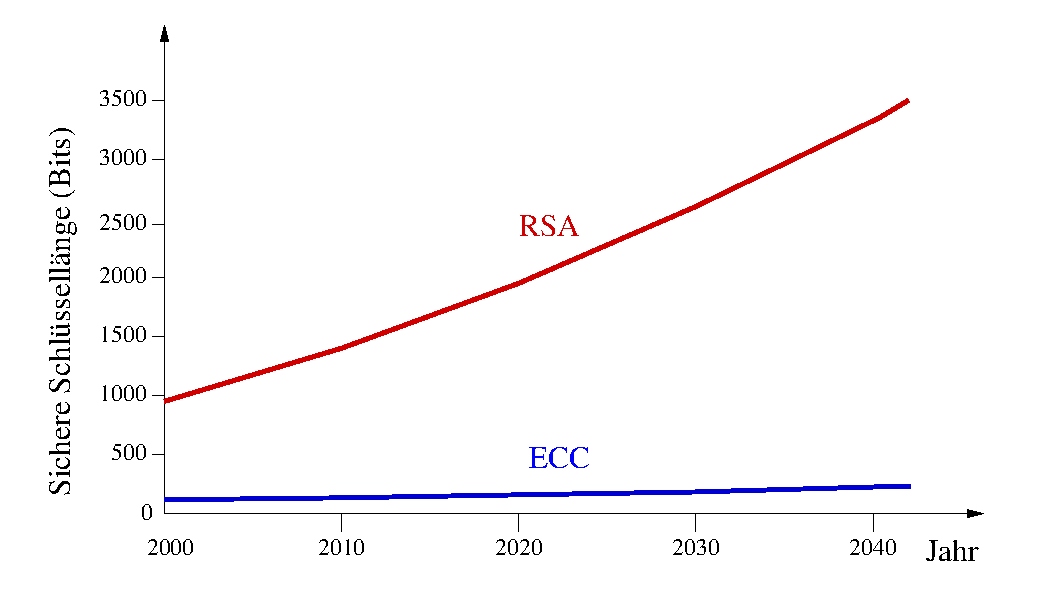
\includegraphics[scale=0.7]{figures/RSAKeyLength-2}
\caption{Prognose f"ur die Entwicklung der als sicher betrachteten
  Schl"ussell"angen f"ur RSA und Elliptische Kurven\vspace{1ex}} 
\label{RSAKeylength}
\end{center}
\vskip -30 pt
\end{figure}

\newpage

Bei der digitalen Signatur muss man differenzieren: f"ur die {\em
  Erstellung} einer digitalen Signatur ben"otigen auf Elliptischen
Kurven basierende Verfahren im Vergleich zu RSA nur gut ein Zehntel des
Rechenaufwandes (66 zu 515 Ganzzahlmultiplikationen). Siehe hierzu
Abbildung~\ref{ThousandBitMultiplications} (Quelle: Dr. J.  Merkle,
Elliptic Curve Cryptography Workshop, 2001). Betrachtet man die f"ur eine
{\em Verifikation} durchzuf"uhrenden Rechenschritte, dreht sich dieses Bild
jedoch zu Gunsten von RSA um (112 zu 17 Ganzzahlmultiplikationen). Der 
Grund liegt darin, dass es bei Verwendung des RSA m"oglich ist, einen sehr 
kurzen Exponent f"ur den "offentlichen Schl"ussel zu w"ahlen, solange der 
private Exponent nur hinreichend lang ist.

% -> Figur 2
\begin{figure}[h]
\vskip -40 pt
\begin{center}
\vspace{1.5cm}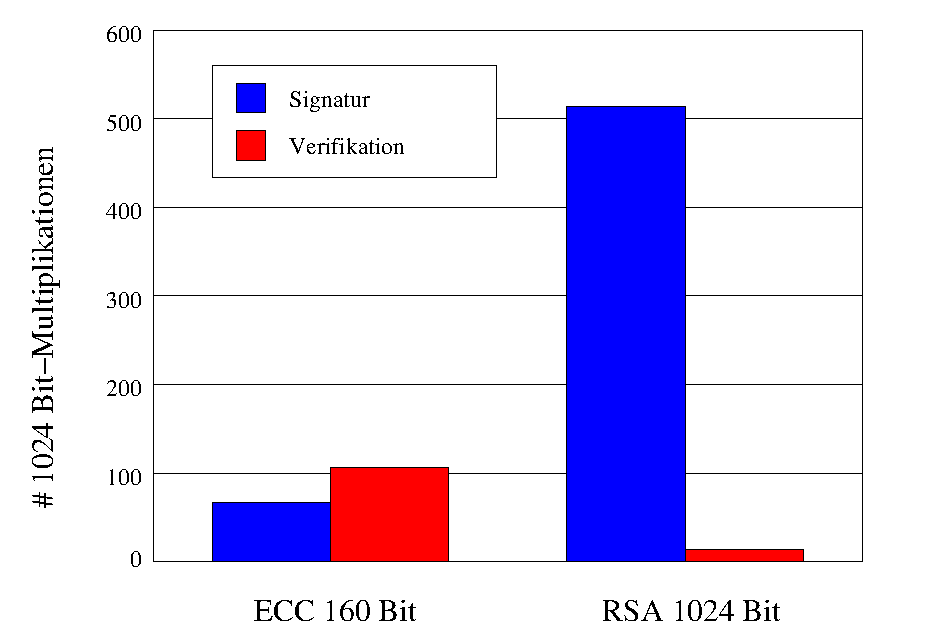
\includegraphics[scale=0.7]{figures/ECCRSA}
\caption{Gegen"uberstellung des Aufwands der Operationen Signieren und Verifizieren bei
  RSA und Elliptischen Kurven} 
\label{ThousandBitMultiplications}
\end{center}
\vskip -10 pt
\end{figure}

Da bei Smartcards, die auf RSA basieren, stets der lange (private)
Schl"ussel auf der Karte gespeichert werden muss und die Erstellung
der digitalen Signatur, nicht aber die Verifikation, auf der Karte
stattfindet, treten hier deutlich die Vorteile Elliptischer Kurven zutage. 
\par
\smallskip
Das gr"o"ste Problem bei der Implementierung von Verfahren, die auf Elliptischen Kurven beruhen, ist bislang die
mangelnde {\em Standardisierung\index{Standardisierung}}. Es gibt nur eine RSA-Implementierung, aber viele Arten, Elliptische Kurven einzusetzen.
So k"onnen verschiedene Zahlk"orper zugrunde gelegt, eine Vielzahl von (Elliptischen) Kurven --- durch
Parameter beschrieben\footnote{%
Siehe Kapitel \ref{ECC-Crypto}
} --- eingesetzt und unterschiedliche Darstellungen der Kurvenpunkte verwendet werden.
Jede Wahl hat ihre Vorz"uge, so dass f"ur jede Anwendung eine andere Implementierung optimal sein kann. Dies
hat jedoch zur Konsequenz, dass Systeme, die auf Elliptischen Kurven beruhen, oftmals nicht interoperabel
sind. Um mit einer beliebigen auf Elliptischen Kurven basierenden Anwendung kommunizieren zu k"onnen, m"usste man
eine Vielzahl von Implementierungen vorhalten, was den Effizienzvorteil gegen"uber der Verwendung von RSA
zunichte macht.

Deshalb bem"uhen sich internationale Organisationen um Standardisierung:
IEEE (P1363), ASC (ANSI X9.62, X9.63), ISO/IEC sowie 
RSA Laboratories\index{RSA Laboratories} und Certicom\index{Certicom}. 
Im Gegensatz zur IEEE, die bisher nur eine Beschreibung der verschiedenen
Implementierungen vorgenommen hat, hat die ASC konkret 10 Kurven ausgew"ahlt
und empfiehlt deren Verwendung. Der Vorteil des ASC-Ansatzes ist,
dass ein einziges Byte ausreicht, um die verwendete Kurve zu spezifizieren.
Zur Zeit ist jedoch nicht absehbar, ob es der ASC gelingen wird, einen
de-facto-Standard durchzusetzen.

Obwohl aktuell kein Handlungsbedarf besteht\footnote{%
Aktuelle Informationen zur Sicherheit des RSA-Verfahrens finden Sie in 
Kapitel \ref{SecurityRSA}.}, laufende RSA-Anwendungen umzustellen, 
sollte man bei der Neuimplementierung ernsthaft den Einsatz von Verfahren
erw"agen, die auf Elliptischen Kurven basieren.
Dies gilt insbesondere, wenn es sich um Anwendungen im Finanzsektor
handelt, die noch nach 2005\footnote{%
BSI-Empfehlung: ``Geeignete Kryptoalgorithmen'' vom 24. Oktober 2002.
} operativ sein sollen.


% -----------------------------------------------------------------------------
\subsection{Elliptische Kurven -- Historisches}

Auf dem Gebiet der Elliptischen Kurven wird seit "uber 100 Jahren geforscht. Im Laufe der Zeit hat man
viele weitl"aufige und mathematisch tiefgr"undige Resultate im Zusammenhang mit Elliptischen Kurven gefunden
und ver"offentlicht. Ein Mathematiker w"urde sagen, dass die Elliptischen Kurven
(bzw.\ die dahinterstehende Mathematik) gut verstanden sind. Urspr"unglich war diese Forschung reine
Mathematik, das hei"st Elliptische Kurven wurden zum Beispiel in den mathematischen Teilgebieten
Zahlentheorie und algebraische Geometrie untersucht, die allgemein sehr abstrakt sind. Auch in der
nahen Vergangenheit spielten Elliptische Kurven eine bedeutende Rolle in der reinen Mathematik. In den
Jahren 1993 und 1994 ver"offentlichte Andrew Wiles\index{Wiles Andrew} mathematische Arbeiten, die weit "uber das Fachpublikum
hinaus auf gro"se Begeisterung gesto"sen sind. In diesen Arbeiten bewies er die Richtigkeit einer --- in
den sechziger Jahren des 20. Jahrhunderts von zwei Japanern aufgestellten --- Vermutung. Dabei geht es
kurz und grob gesagt um den Zusammenhang zwischen Elliptischen Kurven und sogenannten Modulformen.
Das f"ur die meisten eigentlich Interessante daran ist, dass Wiles mit seinen Arbeiten auch den ber"uhmten
zweiten Satz von Fermat\index{Fermat!letzter Satz} bewiesen hat. Dieser Satz hatte sich seit Jahrhunderten
(Fermat\index{Fermat Pierre} lebte von 1601 bis 1665) einem umfassenden Beweis durch die Mathematik entzogen. Dementsprechend
gro"s war die Resonanz auf den Beweis durch Wiles. In der Formulierung von Fermat lautet der nach ihm
benannte Satz so (Fermat hat folgende Worte an den Rand des 1621 von Bachet herausgegebenen Werks Diophants geschrieben):

\begin{quote} {\em
Cubum autem in duos cubos, aut quadratoquadratum in duos quadratoquadratos, et
generaliter nullam in infinitum ultra quadratum potestatem in duos ejusdem nominis
fas est dividere: cujus rei demonstrationem mirabilem sane detexi. Hanc marginis
exiguitas non caperet.
} \end{quote}

Frei "ubersetzt und mit der Schreibweise der heutigen Mathematik bedeutet dies: \\
Es gibt keine positiven ganzen Zahlen $x, y$ und $z$ gr"o"ser als Null, so dass
$x^n + y^n = z^n$ f"ur $n>2$ gilt.
Ich habe einen bemerkenswerten Beweis f"ur diese Tatsache gefunden, aber es ist
nicht genug Platz am Rand [des Buches], um ihn niederzuschreiben.

Dies ist schon bemerkenswert: Eine relativ einfach zu verstehende Aussage
(gemeint ist Fermats zweiter Satz) konnte erst nach so langer Zeit bewiesen werden, obwohl
Fermat selber angab, schon einen Beweis gefunden zu haben.
Im "ubrigen ist der Beweis von Wiles sehr umfangreich (alle im Zusammenhang mit dem Beweis
stehenden Ver"offentlichungen von Wiles ergeben schon ein eigenes Buch). Man sollte sich daher
im klaren sein, dass die Elliptischen Kurven im allgemeinen sehr tiefgreifende Mathematik ber"uhren.

Soweit zur Rolle der Elliptischen Kurven in der reinen Mathematik.
Im Jahr 1985 haben Neal Koblitz\index{Koblitz Neal} und Victor Miller
\index{Miller Victor} unabh"angig voneinander vorgeschlagen, 
Elliptische Kurven in der Kryptographie einzusetzen. Damit haben die 
Elliptischen Kurven auch eine ganz konkrete praktische Anwendung gefunden.
Ein weiteres interessantes Einsatzgebiet f"ur Elliptische Kurven ist die
Faktorisierung von ganzen Zahlen \index{Faktorisierung}
(auf der \index{Komplexit""at} Schwierigkeit/Komplexit"at, die Primfaktoren
einer sehr gro"sen Zahl zu finden, beruht das RSA-Kryptosystem: 
vergleiche Kapitel \ref{SecurityRSA}
). 
In diesem Bereich werden seit 1987 Verfahren untersucht und eingesetzt,
die auf Elliptischen Kurven basieren
(vergleiche Kapitel \ref{ECC-Factorisation}). \\
Es gibt auch Primzahltests\index{Primzahltest}, die auf Elliptischen 
Kurven basieren.
% (s. Anmerkung U. Kuehn)

Elliptische Kurven werden in den verschiedenen Gebieten unterschiedlich
eingesetzt.
Kryptographische Verfahren auf Basis von Elliptischen Kurven beruhen auf der
Schwierigkeit eines als Elliptische Kurven Diskreter Logarithmus bekannten 
Problems.

Ferner gibt es einen Zusammenhang zwischen Faktorisierung von ganzen Zahlen und
Elliptischen Kurven, der in Abschnitt \ref{ECC-Factorisation} n"aher beschrieben 
wird.




% -----------------------------------------------------------------------------
\subsection{Elliptische Kurven -- Mathematische Grundlagen}

In diesem Abschnitt erhalten Sie Informationen "uber
\index{Gruppen} {\em Gruppen} und \index{K""orper} {\em K"orper}.


% -----------------------------------------------------------------------------
\subsubsection{Gruppen}

Da der Begriff der {\em Gruppe} umgangssprachlich anders als in der Mathematik eingesetzt wird, soll der
Vollst"andigkeit halber an dieser Stelle die wesentliche Aussage der formalen Definition einer Gruppe
kurz eingef"uhrt werden:
\begin{itemize}
   \item Eine Gruppe ist eine nichtleere Menge $G$ mit einer Verkn"upfung ``$\cdot$''. Die Menge $G$ ist unter der
         Verkn"upfung $\cdot $ abgeschlossen, d.h, sind $a,b$ Elemente aus $G$, so ist auch ihre Verkn"upfung $ab=a\cdot  b$ ein Element aus $G$.
   \item F"ur alle Elemente $a, b$ und $c$ aus $G$ gilt: $(ab)c = a(bc)$ (Assoziativgesetz).
   \item Es gibt ein Element $e$ in $G$, das sich bez"uglich der Verkn"upfung $\cdot$ neutral verh"alt�, d.h., f"ur alle $a$ aus der Menge $G:$ gilt $ae = ea = a$.
   \item Zu jedem Element $a$ aus $G$ gibt es ein {\it inverses Element}%
\footnote{Das inverse Element ist eindeutig bestimmt, denn sind $x,y\in G$ zwei Inverse zu $a$, d.h. gilt $ax=xa=e$ und $ay=ya=e$, so folgt $x=xe=x(ay)=(xa)y=ey=y$.}
$a^{-1}$(in $G$), so dass gilt: $aa^{-1} = a^{-1}a = e$.
\end{itemize}
Gilt zus"atzlich noch f"ur alle $a, b$ aus $G$, dass $ab = ba$ (Kommutativgesetz), so nennt man die Gruppe $G$ eine {\em abelsche} Gruppe.

% 
Da man auf der selben Menge mehrere Verkn"upfung erkl"aren kann, unterscheidet man diese durch verschiedene Namensgebungen und Zeichen (z.B. $+$ Addition oder $\cdot$ Multiplikation). 

Als einfachstes Beispiel einer (abelschen) Gruppe sei die Gruppe der ganzen Zahlen mit der "ublichen
Addition genannt. Die Menge der ganzen Zahlen wird mit ${\mathbb Z}$ bezeichnet. ${\mathbb Z}$ hat unendlich viele Elemente,
denn ${\mathbb Z} = \{ \cdots, -4, -3, -2, -1, 0, 1, 2, 3, 4, \cdots\}$. Die Verkn"upfung von zum Beispiel $1+2$
liegt in ${\mathbb Z}$, denn $1+2 = 3$ und $3$ liegt in ${\mathbb Z}$. Das neutrale Element der Gruppe
${\mathbb Z}$ ist $0$. Das Inverse Element von $3$ ist $-3$, denn $3+(-3) = 0$.

F"ur unsere Zwecke besonders interessant sind sogenannte {\em endliche} Gruppen, bei denen die zugrundelegte Menge $G$ nur aus einer endlichen Anzahl von
Elementen besteht. Beispiele sind die Gruppen ${\mathbb Z}_n = \{0, 1, 2, 3, \cdots, n-1\}, n$ der Teilerreste bei der Division durch $n$ mit der Addition als Verkn"upfung.

\paragraph{Zyklische Gruppen}\index{Gruppen!zyklische}
Als {\it zyklische Gruppen}\footnote{Zyklische Gruppen k"onnen grunds"atzlich auch unendlich sein wie z.B. die additive Gruppe der ganzen Zahlen. Wir betrachten hier jedoch nur endliche zyklische Gruppen.} bezeichnet man solche Gruppen $G'$, die ein Element $g$ besitzen, aus dem man
mittels der Gruppen-Verkn"upfung alle anderen Elemente der Gruppe erzeugen kann. Es gibt also f"ur jedes
Element $a$ aus $G'$ eine positive, ganze Zahl $i$, so dass die $i$-fache Verkn"upfung von $g$ mit sich
selbst $g^i = g\cdot g \cdots g = a$. Das Element $g$ ist ein {\em Generator} der zyklischen Gruppe --- jedes Element
in $G�$ l"asst sich mittels $g$ und der Verkn"upfung erzeugen.


\paragraph{Ordnung von Elementen einer Gruppe}\index{Gruppen!Ordnung}
Nun zur Ordnung eines Elements der Gruppe: Sei $a$ aus $G$. Die kleinste positive ganze Zahl $r$ f"ur
die gilt, dass $a^r$, also $r$ mal $a$ mit sich selbst verkn"upft, das neutrale Element der Gruppe $G�$ ist
(d.h. $a^r = e$), nennt man {\em Ordnung} von $a$.

Die {\it Ordnung der Gruppe} ist die Anzahl der Elemente in der Menge $G$. Ist die Gruppe $G$ zyklisch und $g$ ein Generator, so stimmt die Ordnung von $g$ mit der Gruppenordnung "uberein. Man kann leicht zeigen, dass die Ordnung eines Gruppenelements stets die Gruppenordnung teilt. Hieraus folgt insbesondere, dass Gruppen mit Primzahlordnung (d.h. die Ordnung der Gruppe ist eine Primzahl) zyklisch sind.


% -----------------------------------------------------------------------------
\subsubsection{K"orper}

In praktischen Anwendungen betrachtet man h"aufig Mengen, auf denen nicht nur eine \mbox{(Gruppen-)}
Verkn"upfung, sondern zwei Verkn"upfungen definiert sind. Diese nennt man oft Addition und Multiplikation. Die mathematisch interessantesten Mengen dieser Art sind sogenannte K"orper, wie z.B. die Menge der reellen Zahlen.

Unter einem K"orper versteht man in der Mathematik eine Menge $K$ mit den zwei Verkn"upfungen Addition und Multiplikation (mit $+$ und $\cdot$ bezeichnet), so dass die folgenden Bedingungen erf"ullt sind:
\begin{itemize}
   \item Die Menge $K$ ist zusammen mit der Verkn"upfung $+$ (Addition) 
         eine abelsche Gruppe. Dabei sei $0$ das neutrale Element der 
	 Verkn"upfung $+$.
   \item Die Menge $K\setminus\{0\}$ (d.h. $K$ ohne das Element 0) ist 
         zusammen mit der Verkn"upfung $\cdot$ (Multiplikation)
         ebenfalls eine abelsche Gruppe. Dabei sei $1$ das neutrale Element
	 der Verkn"upfung $\cdot$.
   \item F"ur alle Elemente $a, b$ und $c$ aus $K$ gilt
         $c\cdot (a+b) = c \cdot a + c \cdot b$ und
         $(a+b) \cdot c = a \cdot c + b \cdot c$ (Distributivgesetz).
\end{itemize}

K"orper k"onnen endlich viele oder unendliche viele Elemente enthalten --- je nach dem nennt man den K"orper {\em endlich} oder {\em unendlich}. So sind die uns vertrauten K"orper der rationalen bzw. der reellen Zahlen unendlich. Beispiele f"ur endliche K"orper sind die Primk"orper
${\mathbb Z}_p = \{0, 1, 2, 3, \cdots, p-1\}$, $p$ eine Primzahl, versehen mit
der Addition modulo $p$ und der Multiplikation modulo $p$ (auch Restklassenk"orper genannt).
\index{K""orper!Charakteristik}
\paragraph{Charakteristik eines K"orpers}
Die Charakteristik eines K"orper $K$ ist die Ordnung des neutralen Elements der Multiplikation ($1$-Element) bez"uglich der Addition, d.h. die kleinste nat"urliche Zahl $n$, so dass gilt
$$ \underbrace{1 + 1 + \cdots + 1}_{\hbox{$n$ mal}} =0
 \, ,
$$
wobei $0$ das neutrale Element der Addition ist.
Gibt es keine solche nat"urliche Zahl, d.h. ergibt $1 + 1 + \cdots + 1$ unabh"angig von der Zahl der Summanden nie das neutrale Element der Addition $0$, so sagt man, der K"orper habe Charakteristik $0$.

K"orper mit Charakteristik $0$ haben daher stets die (paarweise verschiedenen) Elemente $1, 1+1, 1+1+1, \dots$ und sind folglich stets unendlich; andererseits k"onnen K"orper mit endlicher Charakteristik durchaus endlich oder auch unendlich sein.
Ist die Charakteristik $n$ endlich, so muss sie eine Primzahl sein, denn w"are sie zusammengesetzt, d.h. $n=pq$, so sind $p,q<n$ und aufgrund der Minimalit"at der Charakteristik ist keines der K"orperelemente $\bar p=\underbrace{1 + 1 + \cdots + 1}_{\hbox{$p$ mal}}$, $\bar q=\underbrace{1 + 1 + \cdots + 1}_{\hbox{$q$ mal}}$ gleich $0$. Folglich existieren Inverse $\bar p^{-1},\bar q^{-1}$ bez"uglich der Multiplikation. Dann ist aber $(\bar p\bar q)( \bar p^{-1}\bar q^{-1})=1$, andererseits ist nach Definition der Charakteristik $\bar p\bar q=\bar n=\underbrace{1+1+\dots+1}_{\hbox{$n$ times}}=0$ und somit $\underbrace{(\bar p\bar q)}_{=0}( \bar p^{-1}\bar q^{-1})=0$, was zu einem Widerspruch f"uhrt.

Beispiel: Der K"orper ${\mathbb Z}_p$, $p$ prim, hat die Charakteristik $p$. Ist $p$ nicht prim, so ist ${\mathbb Z}_p$ gar kein K"orper.

Der einfachste, denkbare K"orper ist ${\mathbb Z}_2 \; = \{ 0,1\}$, der nur Null- und Einselement enth"alt. Dabei ist $0+0=0$, $0+1=1+0=1$, $1+1=0$, $1\cdot 1=1$, $0\cdot 0=0\cdot 1=1\cdot 0=0$.

\index{K""orper!endliche}
\paragraph{Endliche K"orper}
Wie bereits erw"ahnt, hat jeder endliche K"orper eine Charakteristik $p\ne 0$, wobei $p$ eine Primzahl ist. Zu jeder Primzahl $p$ gibt es einen K"orper mit $p$ Elementen, n"amlich ${\mathbb Z}_p$.

Die Anzahl der Elemente eines K"orpers muss jedoch im allgemeinen keine Primzahl sein. So ist es nicht schwer, einen K"orper mit $4$ Elementen zu konstruieren\footnote{%
Die Menge $K=\{0,1,a,b\}$ ist mit den Verkn"upfungen der folgenden Tabellen ein K"orper:\\
$
\begin{array}{|c||c|c|c|c|} 
\hline 
+ & 0 & 1 & a & b \\
\hline \hline
0 & 0 & 1 & a & b \\
\hline 
1 & 1 & 0 & b & a \\
\hline 
a & a & b & 0 & 1 \\
\hline 
b & b & a & 1 & 0 \\
\hline 
\end{array} \qquad {\rm ~und~} \qquad
\begin{array}{|c||c|c|c|c|} 
\hline 
\cdot & 0 & 1 & a & b  \\
\hline \hline
0 & 0 & 0 & 0 & 0 \\ 
\hline 
1 & 0 & 1 & a & b \\ 
\hline 
a & 0 & a & b & 1 \\ 
\hline 
b & 0 & b & 1 & a \\
\hline 
\end{array} 
$  \\
}.

Man kann zeigen, dass die Ordnung jedes K"orpers eine Primzahlpotenz (d.h. die Potenz einer Primzahl) ist. Andererseits kann man zu jeder Primzahlpotenz $p^n$ einen K"orper konstruieren, der die Ordnung $p^n$~hat. Da zwei endliche K"orper mit gleicher Zahl von Elementen nicht unterscheidbar\footnote{Sind $K,K'$ zwei K"orper mit $k=p^n$ Elementen, so gibt es eine eineindeutige Abbildung $\varphi:K\to K'$, die sich mit der K"orperarithmetik vertr"agt. Eine solche Abbildung nennt man Isomorphie. Isomorphe K"orper verhalten sich mathematisch gleich, so dass es keinen Sinn macht, zwischen ihnen zu unterscheiden. Z.B. sind ${\mathbb Z}_2$ und $K'=\{ NULL,EINS\}$ mit Nullelement $NULL$ und Einselement $EINS$ isomorph. Hierbei sei darauf hingewiesen, dass mathematische Objekte ausschlie"slich "uber ihre Eigenschaften definiert sind.} sind, spricht man von {\bf dem\ K"orper mit $p^n$ Elementen} und bezeichnet diesen mit $GF(p^n)$. Dabei steht $GF$ f"ur {\it Galois Feld} in Erinnerung an den franz"osischen Mathematiker Galois.

Eine besondere Rolle spielen die K"orper $GF(p)$, deren Ordnung eine Primzahl ist. Man nennt solche K"orper Primk"orper zur Primzahl $p$ und bezeichnet ihn meist mit ${\mathbb Z}_p$\footnote{F"ur Primk"orper sind die additive Gruppe sowie die multiplikative Gruppe zyklisch. Ferner enth"alt jeder K"orper $GF(p^n)$ einen zu ${\mathbb Z}_p$ isomorphen Primk"orper.}.

 

% -----------------------------------------------------------------------------
\subsection{Elliptische Kurven in der Kryptographie} \label{ECC-Crypto}

In der Kryptographie betrachten wir Elliptische Kurven. Solche Kurven ergeben sich als L"osungen einer Gleichung der Form\footnote{Die hier verwendete Kurve erh"alt man als Nullstellen des {\it Polynoms}\index{Polynom} $F$ vom Grad drei in drei Variablen. Dabei bezeichnet man allgemein Ausdr"ucke der Form
$P=\sum_{i_1,\dots,i_n\in\N_0} a_{i_1\dots i_n} x_1^{i_1}\dots x_n^{i_n}$ mit Koeffizienten $a_{i_1\dots i_n}\in K$ als Polynome in $n$ Variablen $x_1,\dots,x_n$ "uber dem K"orper $K$, wenn ${\rm grad\,} P:=\max\{i_1+\dots +i_n: a_{i_1\dots i_n}\ne 0\}$ einen endlichen Wert hat, die Summe also nur aus endlich vielen Summanden (Monomen) besteht. Die Summe der Exponenten der Variablen jedes einzelnen Summanden ist maximal $3$, bei mindestens einem Summanden kommt $3$ als Exponentwert einer Variablen auch wirklich vor.}
\begin{equation}
 F(x_1,x_2,x_3)=-x_1^3+x_2^2x_3+a_1x_1x_2x_3-a_2x_1^2x_3+a_3x_2x_3^2-a_4x_1x_3^2-a_6x_3^3=0.
\label{eccbasisgleichung}
\end{equation}
Dabei sind die Variablen $x_1,x_2,x_3$ sowie die Parameter $a_1,\dots,a_4,a_6$ Elemente eines gegebenen K"or"pers $K$. K"orper und Parameter m"ussen so gew"ahlt werden, dass die Kurve bestimmte, f"ur die Kryptographie relevante Eigenschaften besitzt. Der zugrunde liegende K"orper $K$ kann einfach die bekannte Menge der reellen Zahlen oder auch ein endlicher K"orper sein (vgl. letzter Abschnitt).
Damit sich eine sinnvolle Kurve ergibt, m"ussen die Parameter so gew"ahlt sein, dass die folgenden Nebenbedingungen gelten
$$ {\partial F\over\partial x_1}\ne 0, \quad {\partial F\over\partial x_2}\ne 0, \quad
{\partial F\over\partial x_3}\ne 0 .
$$
Ferner betrachten wir Punkte, die sich nur durch eine Vervielfachung jeder Komponente ergeben, als identisch, denn mit $(x_1,x_2,x_3)$ erf"ullt stets auch $\alpha (x_1,x_2,x_3)$ die Ausgangsgleichung. Formal betrachten wir daher "Aquivalenzklassen von Punkten $(x_1,x_2,x_3)$, wobei wir zwei Punkte als gleich ansehen, wenn sie durch Multiplikation mit einer Konstante $\alpha$ auseinander hervorgehen.
\\ Setzt man in der Ausgangsgleichung $x_3=0$, so wird diese zu $-x_1^3=0$, also $x_1=0$. Folglich ist die "Aquivalenzklasse, die das Element $(0,1,0)$ enth"alt, die einzige Punkt mit $x_3=0$. F"ur alle anderen L"osungspunkte k"onnen wir die Transformation
$$ K\times K\times (K\setminus\{0\})\ni (x_1,x_2,x_3) \mapsto (x,y):=\left( {x_1\over x_3}, {x_2\over x_3}\right) \in K\times K
$$
vornehmen, die die Anzahl der Variablen von drei auf zwei reduziert. 
Die Ausgangsgleichung $F(x_1,x_2,x_3)=0$ war so gew"ahlt, dass sich auf
diese Weise die sogenannte Weierstrass-Glei"-chung\footnote{%
Karl Weierstrass\index{Weierstrass, Karl}, 31.10.1815$-$19.12.1897, deutscher Mathematiker, 
Verfechter der streng formalen Ausrichtung der Mathematik.
}
\begin{equation}
 y^2+a_1xy+a_3y = x^3+a_2x^2+a_4x+a_6
\label{ell}
\end{equation}
ergibt.
Da alle bis auf einen L"osungspunkt durch die Gleichung (\ref{ell}) beschrieben werden k"onnen, bezeichnet man (\ref{ell}) auch oft als die Elliptische Gleichung, ihre L"osungsmenge folglich mit
$$ {\bf E} = \left\{(x,y)\in K\times K \, |\, y^2+a_1xy+a_3y = x^3+a_2x^2+a_4x+a_6  \right\} \cup \{{\cal O} \}.
$$
Dabei soll ${\cal O}$ den auf diese Weise nicht beschriebenen Punkt $(0,1,0)$ darstellen, der durch die Projektion (Division durch $x_3$) quasi in den unendlich fernen Punkt abgebildet wird.

\begin{figure}[h]
\begin{center}
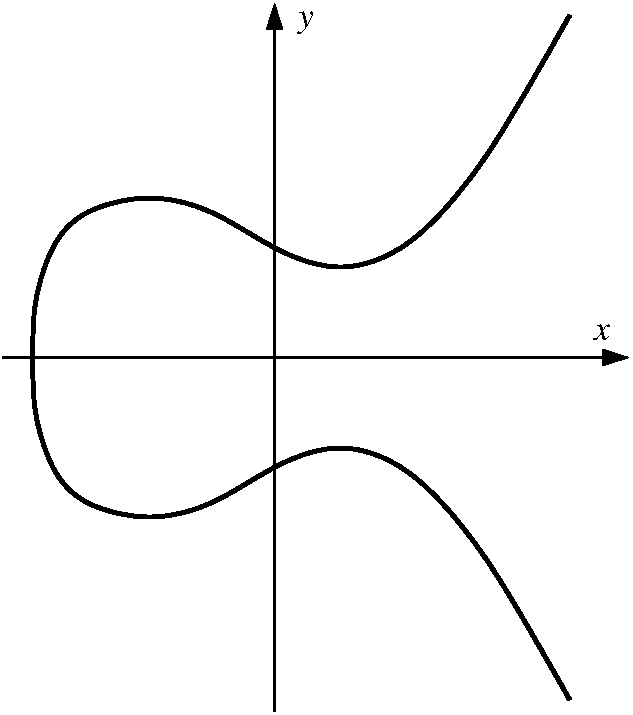
\includegraphics[scale=0.60]{figures/elliptic-curve}
\caption{Beispiel einer Elliptischen Kurve "uber dem K"orper der reellen Zahlen.\vspace{1ex}} 
\label{ExampleEllipticCurve}
\end{center}
\vskip -10 pt
\end{figure}
Als zugrunde liegenden K"orper f"ur eine Elliptische Kurve verwendet man in der Kryptographie stets endliche K"orper $K=GF(p^n)$, also nicht wie in Abbildung \ref{ExampleEllipticCurve} die zu einer stetigen Kurve f"uhrenden reellen Zahlen. Der Grund liegt, einfach gesagt, darin, dass wir bei der Verarbeitung und "Ubertragung von Nachrichten stets nur endlich viele Zust"ande zur Verf"ugung haben (aufgrund der Arbeitsweise moderner Computer), K"orper mit unendlich vielen Elementen wie z.B. die reellen Zahlen daher stets nur unvollst"andig darstellen k"onnen.

In der Praxis hat es sich als sinnvoll erwiesen, entweder $GF(p)$ mit einer gro"sen Primzahl $p$ oder $GF(2^n)$ mit einer (gro"sen) nat"urlichen Zahl $n$ zu betrachten. Der Grund f"ur die Verwendung des Primk"orpers $GF(p)$ liegt in seiner einfachen Arithmetik; andererseits kommt $GF(2^n)$ der bin"aren Darstellung in Computersystemen entgegen. Andere K"orper wie z.B. $GF(7^n)$ bieten keiner dieser beiden Vorteile und werden daher in der Praxis nicht verwendet, ohne dass dies theoretische Gr"unde h"atte.

Durch Koordinatentransformation kann man die Weierstrass-Gleichung\index{Weierstrass, Karl} in einer einfacheren Form schreiben\footnote{Anschaulich bedeutet eine solche Koordinatentransformation eine Drehung bzw. Streckung der Koordinatenachsen, ohne dass die zugrunde liegende Kurve selbst ver"andert wird.}.  Je nachdem, ob $p>3$ ist, verwendet man unterschiedliche Transformationen und erh"alt so

\begin{itemize}
\item im Fall $GF(p)$, $p>3$, die Elliptische Kurven-Gleichung der Form
\begin{equation}
 y^2 = x^3 + ax + b
\label{ellp}
\end{equation}
mit $4a^3+27b^2\ne 0$
\item im Fall $GF(2^n)$ die Elliptische Kurven-Gleichung der Form
\begin{equation}
 y^2+xy = x^3 + ax^2 + b
\label{ell2}
\end{equation}
mit $b\ne 0$\footnote{Die Form (\ref{ellp}) ist die Standardform der Weierstrass-Gleichung\index{Weierstrass, Karl}. Ist die Charakteristik des K"orpers jedoch $2$ oder $3$, so ist $4=0$ bzw. $27=0$, was dazu f"uhrt, dass man in der Bedingung an die Parameter $a,b$ wesentliche Informationen verliert. Dies ist ein Hinweis darauf, dass die Transformation auf die Standardform in diesen F"allen nicht zu befriedigenden Ergebnissen f"uhrt.}.
\end{itemize}
Durch diese Bedingungen an die Parameter $a,b$ ist gew"ahrleistet, dass die Elliptische Gleichung f"ur kryptographische Anwendungen geeignet ist\footnote{Formal sagt man, die Kurve ist nicht singul"ar.}.



F"ur die Anzahl $|E|$ der Elemente einer Elliptischen Kurve $E$ "uber einem K"orper $GF(k)$ (praktisch $k=p$ prim oder $k=2^n$) gilt nach dem Satz von Hasse \cite{Silverman1986} die einfache Beziehung $| \, |E| - k-1\,| \le 2\cdot \sqrt{k}$. Diese Ungleichung ist "aquivalent zu $k+1 - 2\sqrt{k} < |E| < k+1+2\sqrt{k}$. Dies bedeutet, dass die Anzahl der Elemente der Elliptischen Kurve mit der Gr"o"se $k$ gut abgesch"atzt werden kann. 

% $$ (\sqrt{k}-1)^2=k-2\sqrt{k}+1 \le |E| \le k+1 .
% $$
% Dies bedeutet, dass f"ur gro"se $k$ die Anzahl der Elemente der Elliptischen Kurve praktisch wie $k$ w"achst.


% -----------------------------------------------------------------------------
\subsection{Verkn"upfung auf Elliptischen Kurven}

Um mit Elliptischen Kurven arbeiten zu k"onnen, definiert man eine Verkn"upfung (meist additiv als $+$ geschrieben) auf den Punkten der Elliptischen Kurve. Dabei definiert man bei Elliptischen Kurven "uber $GF(p)$ die kommutative Verkn"upfung durch
\begin{enumerate}
\item $P+{\cal O}={\cal O}+P=P$ f"ur alle $P\in E$,
\item f"ur $P=(x,y)$ und $Q=(x,-y)$ ist $P+Q={\cal O}$,
\item f"ur $P_1=(x_1,x_2),P_2=(x_2,y_2)\in E$ mit $P_1,P_2\ne {\cal O}$ und $(x_2,y_2)\ne (x_1,-y_1)$ ist $P_3:=P_1+P_2$, $P_3=(x_3,y_3)$ definiert durch
$$ x_3:=-x_1-x_2+\lambda^2 \, , \qquad y_3:=-y_1+\lambda (x_1-x_3)
$$
mit dem Hilfsquotienten
$$ \lambda:=\left\{ \begin{array}{cl} {y_1-y_2\over x_1-x_2} & {\rm falls~} P_1\ne P_2, \\
                                     {3x_1^2+a\over 2y_1} & {\rm falls~} P_1=P_2. \end{array} \right.
$$
\end{enumerate}
Hieraus folgt insbesondere f"ur $P=(x,y)\in E$, dass gilt $-P=(x,-y)$.

"Uber $GF(2^n)$ definiert man analog die Verkn"upfung durch
\begin{enumerate}
\item $P+{\cal O}={\cal O}+P=P$ f"ur alle $P\in E$,
\item f"ur $P=(x,y)$ und $Q=(x,x+y)$ ist $P+Q={\cal O}$,
\item f"ur $P_1=(x_1,x_2),P_2=(x_2,y_2)\in E$ mit $P_1,P_2\ne {\cal O}$ und $(x_2,y_2)\ne (x_1,x_1+y_1)$ ist $P_3:=P_1+P_2$, $P_3=(x_3,y_3)$ definiert durch
$$ x_3:=-x_1+x_2+\lambda+\lambda^2+a \, , \qquad y_3:=y_1+x_3+\lambda (x_1+x_3)
$$
mit
$$ \lambda:=\left\{ \begin{array}{cl} {y_1+y_2\over x_1+x_2} & {\rm falls~} P_1\ne P_2, \\
                                   x_1+{y_1\over x_1} & {\rm falls~} P_1=P_2. \end{array}\right.
$$
\end{enumerate}
Hieraus folgt insbesondere f"ur $P=(x,y)\in E$, dass gilt $-P=(x,x+y)$. (Beachte: $-(-P)=(x,x+(x+y))=(x,2x+y)=(x,y)$, da der zugrunde liegende K"orper Charakteristik $2$ hat.)\footnote{Eine Animation der Punktaddition auf Elliptischen Kurven 
findet man auf der Certicom-Seite\index{Certicom} unter \\
\href{http://www.certicom.com/resources/ecc_tutorial/ecc_tutorial.html}{\texttt{http://www.certicom.com/resources/ecc\_tutorial/ecc\_tutorial.html}}}

Man kann nachrechnen, dass die Menge $E\cap\{\cal O\}$ mit der so definierten
Addition eine Gruppe bildet. Dies bedeutet insbesondere, dass die Summe zweier
Kurvenpunkte stets wieder ein Punkt auf der Elliptische Kurve ist. Diese
Addition l"a"st sich auch geometrisch veranschaulichen, wie der folgende
Abschnitt zeigt.

% \newpage
\begin{figure}[htbp]
\subsubsection*{Addieren von Punkten auf einer Elliptischen Kurve}
Die zwei folgenden Abbildungen zeigen, wie bei einer Elliptischen Kurve "uber den reellen Zahlen in affinen Koordinaten
zwei Punkte addiert werden. Der unendlich ferne Punkt ${\cal O}$ kann nicht in der affinen 
Ebene dargestellt werden.  
\begin{center}
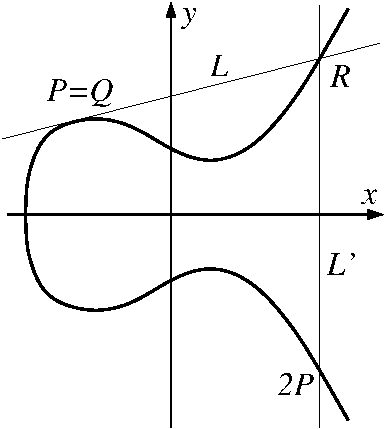
\includegraphics[scale=1.08]{figures/ec-mult2}
\caption{Verdoppelung eines Punktes} 
\vspace{\floatsep}
\vskip +20 pt
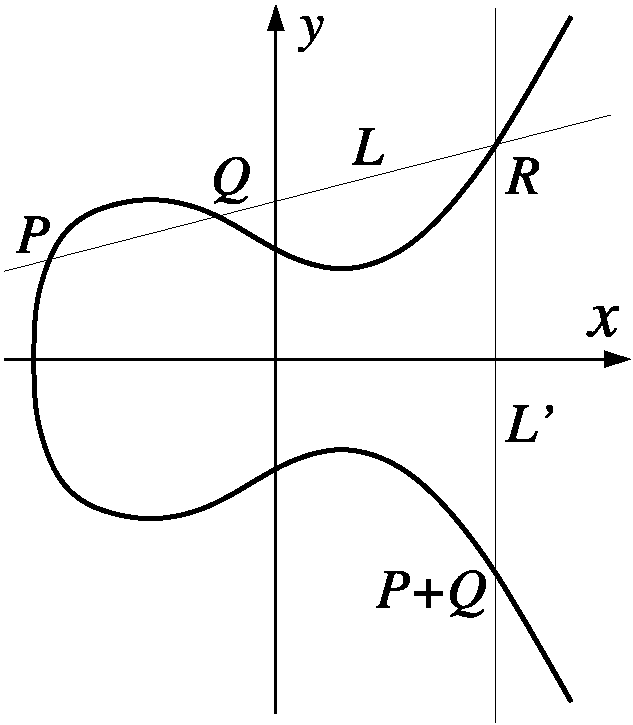
\includegraphics[scale=0.65]{figures/ec-add}
\caption{Addition zweier verschiedener Punkte im K"orper der reellen Zahlen} % \footnotemark }
\end{center}
\end{figure}
% \addtocounter{footnote}{0}\footnotetext{Der Punkt $O$ kann nicht in der affinen Ebene dargestellt werden.}
\enlargethispage{+20pt}
\newpage


% -----------------------------------------------------------------------------
\subsection{Sicherheit der Elliptischen-Kurven-Kryptographie: Das ECDLP}

Wie bereits in Abschnitt \ref{ECC-Crypto} erw"ahnt, betrachten wir in der Kryptographie Elliptische Kurven "uber diskreten\footnote{Diskret im Gegensatz zu kontinuierlich.} K"orpern $GF(2^n)$ oder $GF(p)$ (f"ur gro"se Primzahlen $p$). Dies bedeutet, dass alle Parameter, die zur Beschreibung der Elliptischen Kurve notwendig sind, aus diesem zugrunde liegenden K"orper stammen. Ist nun $E$ eine Elliptische Kurve "uber einem solchen K"orper und $P$ ein Punkt auf der Kurve $E$, so kann man f"ur jede nat"urliche Zahl $m$
$$ mP := \underbrace{P+P+\dots+P}_{\hbox{$m$ mal}}
$$
bilden. Diese Operation ist aus kryptographischer Sicht deshalb besonders interessant, weil man einerseits um $mP$ zu berechnen im allgemeinen nur $\log m$ Additionen durchf"uhren muss --- man bildet einfach $P$, $2P$, $2^2P$, $2^3P$, \dots, schreibt $m$ bin"ar und addiert schlie"slich entsprechend der Bin"ardarstellung von $m$ auf --- es andererseits sehr aufwa"ndig zu sein scheint, zu gegebenen Punkten $P$ und $Q=mP$ auf $E$ die Zahl $m$ zu bestimmen. Nat"urlich kann man $P,2P,3P,4P,5P,\dots$ bilden und jeweils mit $Q$ vergleichen. Hierzu ben"otigt man jedoch $m$ Additionen.

Bisher ist noch kein Algorithmus bekannt, der effizient $m$ aus $P$ und $Q$ berechnet. Die bisher besten Verfahren liegen z.B. im Fall $GF(p)$ in der Gr"o"senordnung $\sqrt{q}$, wobei $q$ ein (gro"ser) Primfaktor von $p-1$ ist; $m$ selbst sollte in diesem Fall zwischen $1$ und $q$ liegen, so dass man f"ur die Muliplikation $mP$ maximal $\log q$ Schritte ben"otigt. Der Quotient ${\sqrt{q}\over\log q}$ strebt jedoch (schnell) gegen $+\infty$.

Sind die Parameter hinreichend gro"s (ist zum Beispiel $p$ prim und
mehr als $160$ Bit lang) ist der Computer ohne weiteres in der Lage, sehr schnell (in wenigen
Bruchteilen einer Sekunden) den Punkt $mP$ zu bestimmen. Das {\it inverse Problem}, $m$ aus $mP$ und $P$ zu erhalten, ist jedoch nicht in akzeptabler Zeit m"oglich.

Dies wird als das \glqq Diskrete Logarithmus Problem "uber Elliptischen Kurven\grqq\ bezeichnet
(auch ECDLP\index{ECDLP} - Elliptic Curve Discrete Logarithm Problem - abgek"urzt).

\vskip +5 pt

Formal betrachten wir in der Elliptischen-Kurven-Kryptographie die Punkte der Kurve als Elemente einer Gruppe mit der Addition als Verkn"upfung. Allerdings sind nur solche Elliptischen Kurven f"ur kryptographische Anwendungen geeignet, bei der die Anzahl der Kurvenpunkte hinreichend gro"s ist. Ferner k"onnen in Spezialf"allen Elliptische Kurven auch aus anderen Gr"unden ungeeignet sein. Das bedeutet, dass man bei der
Definition einer Kurve auf die Wahl der Parameter achten muss. Denn f"ur bestimmte Klassen von
Elliptischen Kurven ist es m"oglich, das ECDLP leichter zu l"osen als im allgemeinen Fall. Kryptographisch
ungeeignete Elliptische Kurven sind die sogenannten {\em anormalen} Kurven (das sind Kurven "uber ${\mathbb Z}_p$,
f"ur die die Menge ${\bf E}$ genau $p$ Elemente hat) und die {\em supersingul"aren} Kurven (das sind Kurven, f"ur die man das
Berechnen des ECDLP auf das Berechnen des \glqq normalen\grqq\ Diskreten Logarithmus in anderen endlichen K"orper
reduzieren, d.h. vereinfachen, kann). Daher gibt es kryptographisch gute und schlechte Kurven. Allerdings
kann man f"ur gegebene Parameter $a$ und $b$ mit etwas Aufwand feststellen, ob die resultierende Elliptische
Kurve kryptographisch brauchbar ist oder nicht. Die in der Kryptographie eingesetzten Kurven werden meist
von Fachleuten zur Verf"ugung gestellt. Sie gew"ahrleisten, dass die von ihnen als sicher eingestuften
Elliptischen Kurven den aktuellen Sicherheitsanforderungen gen"ugen.
\vskip +5 pt

Bei sicheren Kurven wird haupts"achlich
durch den Parameter $p$ im Fall des zugrunde liegenden K"orpers $GF(p)$ bzw. $n$ im Fall des zugrunde liegenden K"orpers $GF(2^n)$ bestimmt, wie lange es dauert, das ECDLP auf dieser Kurve zu l"osen. Je gr"o"ser diese
Parameter sind, desto l"anger nimmt das L"osen des Problems in Anspruch. Von Fachleuten wird z.B. eine Bitl"ange
von "uber $200$ Bit f"ur den Parameter $p$ empfohlen. Hier wird deutlich, warum die Elliptischen Kurven so
interessant f"ur die Kryptographie sind. Denn die Parameter bestimmen auch den
Signatur-/Verschl"usselungsaufwand, wenn mit Elliptischen Kurven
Kryptographie betrieben wird. Die Dauer einer Schl"usselpaar-Erzeugung ist ebenfalls von den Parametern abh"angig. Daher sind kleine Werte (wenige Bits) w"unschenswert (m"oglichst schnelle Laufzeiten der Verfahren);
allerdings muss die geforderte Sicherheit dabei eingehalten werden. Mit einer L"ange von zum Beispiel $200$ Bit
f"ur $p$ ist eine {\em gute} Elliptische Kurve genau so sicher wie ein \index{RSA!Modulus} RSA-Modulus von "uber $1024$ Bit L"ange
(zumindest nach dem heutigen Forschungstand). Der Grund daf"ur ist, dass die schnellsten Algorithmen zum
L"osen des {\em Elliptische Kurven Diskreter Logarithmus} Problems eine exponentielle Laufzeit haben --- im
Gegensatz zu den subexponentiellen Laufzeiten, die die zur Zeit besten Faktorisierungsalgorithmen haben
(Zahlk"orpersieb, Quadratisches Sieb oder Faktorisieren mit Elliptischen Kurven). Dies erkl"art, warum die
Parameter von Kryptoverfahren, die auf dem Problem {\em Faktorisieren von ganzen Zahlen} beruhen, gr"o"ser sind als
die Parameter von Kryptoverfahren, die auf dem ECDL-Problem basieren.


% -----------------------------------------------------------------------------
\subsection{Verschl"usseln und Signieren mit Hilfe Elliptischer Kurven}

\begin{sloppypar}
  Das {\em Elliptische Kurven Diskreter Logarithmus
    Problem}\index{Logarithmusproblem} (ECDLP) \index{ECDLP} ist die
  Grundlage f"ur die Elliptische-Kurven-Kryptographie. Darauf basierend gibt es verschiedene Signaturverfahren. Um ein solches Signaturverfahren anzuwenden, ben"otigt man:
\end{sloppypar}
\begin{itemize}
    \item Eine Elliptischen Kurve {\bf E}, beschrieben durch den zugrunde liegenden K"orper $GF(p^n)$.
    \item Eine Primzahl $q\ne p$ sowie einen Punkt $G$ auf der Elliptischen Kurve ${\bf E}$ mit Ordnung $q$. D.h., es gilt $qG={\cal O}$ und $rG\ne {\cal O}$ f"ur alle $r\in \{1,2,\dots,q-1\}$. Die Zahl $q$ muss dann ein Teiler der Gruppenordnung (entspricht der Anzahl der Elemente) $\#{\bf E}$ sein. Aufgrund der Primordnung, erzeugt $G$ eine zyklischen Untergruppe von ${\bf E}$ mit Ordnung $q$.
\end{itemize}
Die genannten Parameter bezeichnet man als \index{Domain-Parameter} {\em Domain}-Para\-meter. Durch sie wird
festgelegt, auf welcher Elliptischen Kurve ${\bf E}$ und in welcher zyklischen Untergruppe von ${\bf E}$ ein
Signaturverfahren eingesetzt  wurde.

\par
%\smallskip
%{\bf Verschl"usselung:}
\subsubsection{Verschl"usselung}

Mit Hilfe Elliptischer Kurven kann ein sicherer Schl"usselaustausch nach dem \hyperlink{DH-KeyExch}{Diffie-Hellman} Protokoll \index{Diffie-Hellman} erfolgen (siehe Kapitel \ref{DH-KeyExch}). Dieser Schl"ussel kann dann f"ur eine anschlie"sende symmetrische Verschl"usselung verwendet werden. Ein Schl"usselpaar mit privatem und "offentlichem Schl"ussel wird im Gegensatz zum RSA-Algorithmus hingegen nicht erzeugt!

In der Schreibweise der Elliptischen Kurven liest sich das Diffie-Hellman Verfahren wie folgt: Zun"achst einigen sich beide Partner (A und B) "offentlich auf eine Gruppe $G$ und eine ganze Zahl $q$. Danach w"ahlen sie zuf"allig $r_A,r_B\in\{1,2,\dots,q-1\}$, bilden die Punkte $R_A=r_AG$, $R_B=r_BG$ auf der Elliptischen Kurve und tauschen diese aus. Danach berechnet A leicht $R=r_AR_B$. Denselben Punkt (n"amlich $r_Ar_B G$) erh"alt auch B, indem er $r_BR_A=r_Br_AG=r_Ar_BG=R$ bildet. Dabei ist die Berechnung von $R_A,R_B$ als $r_A$ bzw. $r_B$-faches des Kurvenpunktes $G$ leicht durchzuf"uhren; die umgekehrte Operation, aus $R_A$ bzw. $R_B$ den Wert $r_A$ bzw. $r_B$ zu erhalten, ist jedoch sehr aufw"andig.
\\ F"ur einen Dritten ist es nach heutigen Kenntnisstand nicht m"oglich, $R$ zu berechnen, wenn er nicht mindestens einen der Werte $r_A$ oder $r_B$ ermitteln kann, d.h. das ECDLP l"ost.

Um einen ``Man-in-the-middle''-Angriff zu verhindern, kann man auch hier wie schon in Kapitel \ref{Impersonalisierungsattacke} beschrieben, die "ubertragenen Werte $G,q,R_A,R_B$ digital signieren.

\par
%\smallskip 
%{\bf Signatur-Erstellung:}
\subsubsection{Signatur-Erstellung}

"Ubertr"agt man den \index{DSA} DSA auf Elliptische Kurve, so kann man wie folgt eine digitale Signatur erzeugen: Man w"ahlt vorab eine (nicht-triviale) Zahl $s\in{\mathbb Z}_q$. Diese bildet den privaten Schl"ussel. Hingegen werden $q$, $G$ und $R=sG$ ver"offentlicht. Aus $G$ und $R$ l"asst sich jedoch $s$ nicht ermitteln, worauf die Sicherheit des Signaturverfahrens beruht.

F"ur eine Nachricht $m$ wird zun"achst mit Hilfe eines Hash-Verfahrens $h$ ein digitaler Fingerabdruck erstellt, wobei $h(m)$ im Wertebereich $\{0,1,2,\dots, q-1\}$ liegt und $h(m)$ somit als Element von ${\mathbb Z}_q$ interpretiert werden kann. Dann wird ein zuf"alliges $r\in{\mathbb Z}_q$ gew"ahlt und $R=(r_1,r_2)=rG$ berechnet. Die erste Komponente $r_1$ von $R$ ist ein Element von $GF(p^n)$. Diese wird auf ${\mathbb Z}_q$ abgebildet, z.B. im Fall $n=1$ als Element von $\{0,1,\dots,p-1\}$ interpretiert und dann der Teilerrest modulo $q$ gebildet. Das so erhaltene Element von ${\mathbb Z}_q$ bezeichnen wir mit $\bar r_1$. Nun bestimmt man $x\in {\mathbb Z}_q$ mit
$$ rx-s\bar r_1-h(m)=0 .
$$
Das Tripel $(m,r_1,x)$ bildet nun die digitale Signatur.

\par
%\smallskip 
%{\bf Signatur-Verifikation:}
\subsubsection{Signatur-Verifikation}

Zur Verifikation muss zun"achst $u_1=h(m)/x$, $u_2=\bar r_1/x$ (in ${\mathbb Z}_q$ gebildet werden). Dann bestimmt man
$$ V=u_1G+u_2Q .
$$
Wegen $Q=sG$ ist $V=(v_1,v_2)$ mit $v_1=u_1+u_2s$. Diese Addition findet formal im Raum $GF(p^n)$ statt. Die Projektion von $GF(p^n)$ auf ${\mathbb Z}_q$ sollte jedoch so gew"ahlt sein, dass $\bar v_1=u_1+u_2s$ in ${\mathbb Z}_q$ ist.
Dann gilt n"amlich
$$ \bar v_1=u_1+u_2s=h(m)/x+\bar r_1 s/x=(h(m)+\bar r_1s)/x=rx/x=r .
$$
Nun ist $R=rG$. Also folgt hier $\bar v_1=\bar r_1$, d.h. $R$ und $V$ stimmen modulo der Projektion auf ${\mathbb Z}_q$ "uberein.


% -----------------------------------------------------------------------------
\subsection{Faktorisieren mit Elliptischen Kurven} \label{ECC-Factorisation} 
\hypertarget{faktell}{}

Es gibt Faktorisierungsalgorithmen%
\footnote{Insbesondere John M. Pollard \index{Pollard John M.} war an der 
Entwicklung vieler verschiedener Faktorisierungsalgorithmen beteiligt; auch
beim Faktorisieren mit ECC war er einer der f"uhrenden K"opfe. Als Mitarbeiter
von British Telekom hat er leider nie viel selbst publiziert. Auf der RSA
Konferenz 1999 wurde er f"ur seine \glqq outstanding contributions in 
mathematics\grqq ~ausgezeichnet: 
\href{http://www.eff.org/Privacy/Crypto_misc/DESCracker/HTML/19990118_rsa_awards.html}
{\texttt{http://www.eff.org/Privacy/Crypto\_misc/DESCracker/HTML/19990118\_rsa\_awards.html}}.
}, die auf Elliptischen Kurven \index{Faktorisierung!Faktorisierungsalgorithmen}
basieren\footnote{Im Jahr 1987 stellte H.W. Lenstra\index{Lenstra 1987}
einen Faktorisierungsalgorithmus vor, der auf Elliptischen Kurven basiert 
(siehe \cite{Lenstra1987}). Die aktuell gr"o"ste mit Elliptischen Kurven 
faktorisierte Zahl\index{Faktorisierung!Faktorisierungsrekorde} ist die 
55 Dezimalstellen lange Zahl $629^{59}-1$, sie wurde am 6. Oktober 2001 
von M. Izumi gefunden (siehe \hyperlink{Lenstra2}{ECMNET}\index{ECMNET}).
}.
Genauer gesagt, machen sich diese Verfahren zunutze, dass man auch 
"uber ${\mathbb Z}_n$ ($n$ zusammengesetzte Zahl) Elliptische Kurven
definieren kann. Elliptische Kurven "uber ${\mathbb Z}_n$ bilden keine
Gruppe, da es nicht zu jedem Punkt auf solchen Elliptischen Kurven einen
inversen Punkt geben muss. Dies h"angt damit zusammen, dass es -- falls $n$ 
eine zusammengesetzte Zahl ist -- in ${\mathbb Z}_n$ Elemente gibt, die 
kein Inverses bez"uglich der Multiplikation modulo $n$ haben. Um zwei 
Punkte auf einer Elliptischen Kurve "uber ${\mathbb Z}_n$ zu addieren, kann
prinzipiell genauso gerechnet werden wie auf Elliptischen Kurven "uber
${\mathbb Z}_p$. Eine Addition von zwei Punkten (auf einer Elliptischen
Kurve "uber ${\mathbb Z}_n$) scheitert aber genau dann, wenn man einen 
Teiler von $n$ gefunden hat. Der Grund daf"ur ist, dass das Verfahren zum
Addieren von Punkten auf Elliptischen Kurven Elemente in ${\mathbb Z}_n$ 
ermittelt und zu diesen Elementen die inversen Elemente (bez"uglich der
Multiplikation modulo $n$) in ${\mathbb Z}_n$ berechnet. Dazu wird der
erweiterte \index{Euklidscher Algorithmus} Euklidsche Algorithmus benutzt.
Ergibt sich nun bei der Addition zweier Punkte (die auf einer Elliptischen
Kurve "uber ${\mathbb Z}_n$ liegen) ein Element aus ${\mathbb Z}_n$, das
kein inverses Element in ${\mathbb Z}_n$ hat, so gibt der erweiterte
Euklidsche Algorithmus\index{Euklidscher Algorithmus!erweiterter}
einen echten Teiler von $n$ aus.

Das Faktorisieren mit Elliptischen Kurven funktioniert somit prinzipiell so: Man w"ahlt zuf"allige Kurven
"uber ${\mathbb Z}_n$, sowie zuf"allig irgendwelche Punkte (die auf diesen Kurve liegen) und addiert diese; dabei
bekommt man wieder Punkte, die auf der Kurve liegen oder findet einen Teiler von $n$. Die
Faktorisierungsalgorithmen auf Basis von Elliptischen Kurven arbeiten also probabilistisch.
Durch die M"oglichkeit, sehr viele Elliptische Kurven "uber ${\mathbb Z}_n$ zu definieren, kann man die
Wahrscheinlichkeit erh"ohen, zwei Punkte zu finden, bei deren Addition ein Teiler von $n$ gefunden wird.
Daher eignen sich diese Verfahren auch sehr gut f"ur eine Parallelisierung.


% -----------------------------------------------------------------------------
\subsection{Implementierung Elliptischer Kurven}

CrypTool benutzt Elliptische Kurven bei der Funktion f"ur digitale Signaturen.

Implementiert sind die Basisalgorithmen f"ur Gruppenoperationen, f"ur das Erzeugen von Elliptischen
Kurven und f"ur das Ein- und Auslesen von Parametern f"ur Elliptische Kurven "uber endlichen
K"orpern $GF(p)$ mit $p$ ($p$ prim) Elementen. Die Implementierung erfolgte in ANSI C und richtete sich
nach dem Entwurf Nr.8 der Arbeitsgruppe IEEE P1363 {\em Standard Specifications for Public Key Cryptography}

{\href{http://grouper.ieee.org/groups/1363}{\texttt{http://grouper.ieee.org/groups/1363}}}.

Implementiert sind die kryptographischen Primitive zur Signaturerzeugung und Signaturverifikation f"ur
die auf Elliptischen Kurven basierenden Varianten von Nyberg-Rueppel-Signaturen und \index{DSA} DSA-Signaturen
(nach Entwurf Nr.8 der Arbeitsgruppe IEEE P1363). Dies erfolgte in Zusammenarbeit mit der Secude
GmbH --- und unter Benutzung des Secude SDK.
\index{Secude GmbH}

Wenn man statt des Primk"orpers $GF(p)$ einen K"orper der Form $GF(2^n)$ zugrunde legt, ergeben sich wesentliche Unterschiede in der Implementierung. Der Vorteil einer Implementierung unter Verwendung von $GF(2^n)$ liegt darin, dass Rechnungen aufgrund der bin"aren Darstellung effizienter durchgef"uhrt werden k"onnen. Dies betrifft insbesondere die Division, die in $GF(p)$ vergleichsweise aufw"andig ist (was z.B. bei dem oben beschriebenen Signaturverfahren sowohl die Erstellung der Signatur als auch ihre sp"atere Verifikation betrifft, da beide eine Divisionsoperation enthalten).

Um das Potenzial der Effizienzsteigerung m"oglichst optimal zu nutzen, kann man z.B. K"orper w"ahlen, die besondere Basen besitzen, wie Polynomialbasen (besonders geeignet f"ur Software-Implementierungen) oder Normalbasen (bevorzugt bei Hardware-Implementierungen). F"ur bestimmte Werte von $n$ (wie z.B. $n=163,179,181$) lassen sich sogar beide Vorteile kombinieren. Allerdings sind spezielle Darstellungen oft nicht Standard.

Um Speicherplatz zu sparen, wird zuweilen nur die erste Komponente sowie ein weiteres Bit f"ur jeden Punkt auf der Elliptischen Kurve gespeichert. Hieraus kann jeweils der gesamte Punkt errechnet werden. Dies ist besonders bei Verwendung von Normalbasen effizient. Selbst bei der Durchf"uhrung der kryptographischen Protokolle kann eine signifikante Beschleunigung erreicht werden. Diese sogenannte {\it Punkt-Kompression}, die bei der H"alfte aller Kurven einsetzbar ist, ist jedoch patentiert (US Patent 6141420, Certicon) und daher nicht ohne weiteres frei einsetzbar.

Im allgemeinen Fall $GF(p^n)$ (aber auch f"ur $n=1$) werden oft sogenannte affine oder projektive Koordinaten eingesetzt, was je nach Anwendung zu Effizienzgewinnen f"uhrt.

Eine vollst"andige Beschreibung aller Implementierungen unter Abw"agung ihrer Vor- und Nachteile w"urde an dieser Stelle zu weit f"uhren. Abschlie"send kann festgehalten werden, dass die Vielfalt m"oglicher Implementierungen bei Elliptischen Kurven z.B. im Vergleich zu RSA-Implementie"-rungen sehr gro"s ist. Aus diesem Grund gibt es Bestrebungen, sich auf wenige Standardimplementierungen, ja sogar auf eine kleine Schar fest vorgegebener Kurven zu beschr"anken (ASC-Ansatz).

Der Erfolg dieser Standardisierungsbem"uhungen ist heute noch nicht absehbar.
Dies w"are aber eine Voraussetzung daf"ur, dass sich ECC dauerhaft als
Alternative zu RSA etabliert. Die Arbeit der Standardisierungskomitees wird
sich erheblich beschleunigen m"ussen, wenn sich abzeichnet, dass die aktuellen
Forschungsprojekte im Bereich der Faktorisierung einen Durchbruch erzielen.

% -----------------------------------------------------------------------------
\subsection{Elliptische Kurven im praktischen Einsatz}

Bereits heute werden Elliptische Kurven in der Praxis eingesetzt. Als prominentes Beispiel ist hier der Informationsverbund Bonn-Berlin (IVBB)\footnote{Der IVBB verbindet Regierungsstellen in der alten und neuen deutschen Hauptstadt.}\index{IVBB} zu nennen, bei dem streng vertrauliche Dokumente der deutschen Bundesregierung zwischen Regierungsstellen mit Sitz in Berlin und Bonn ausgetauscht werden. Durch den Einsatz von ECC konnte eine Hochsicherheitsl"osung realisiert werden. Fragen der Interoperabilit"at spielten hingegen eine untergeordnete Rolle.

Nach Auskunft des Projektleiters e-Government in "Osterreich, Prof.\ Posch, ist in K"urze auch mit einer Massenanwendung in "Osterreich auf Basis von ECC zu rechnen: Die Bankkarte mit Signaturanwendung, die ab 2004 herausgegeben werden soll, setzt auf Elliptische Kurven.

Beide Beispiele zeigen gut die typischen Einsatzgebiete Elliptischer Kurven: Als Hochsicherheitsl"osungen und bei Implementierungen auf Smartcards, bei denen der Schl"ussell"ange (Speicherplatz) eine entscheidende Bedeutung zukommt.


\newpage
\begin{thebibliography}{99999}
\addcontentsline{toc}{subsection}{Literaturverzeichnis}
    \bibitem[Cassels1991]{Cassels1991} J. W. S. Cassels,
	\index{Cassels 1991} \\ 
	{\em Lectures on elliptic curves}, \\
	Cambridge University Press, 1991, 143 Seiten.
    \bibitem[Koblitz1984]{Koblitz1984}N. Koblitz, 
	\index{Koblitz 1984} \\
	{\em Introduction to elliptic curves and modular forms}, \\
	Graduate Texts in Mathemathics, Springer-Verlag, 1984.
    \bibitem[Koblitz1998]{Koblitz1998}N. Koblitz, 
	\index{Koblitz 1998} \\
	{\em Algebraic aspects of Cryptography. With an appendix on 
	Hyperelleptic curves by Alfred J. Menezes, Yi Hong Wu and Robert 
	J. Zuccherato}, \\
	Springer-Verlag, 1998, 206 Seiten.
    \bibitem[Menezes1993]{Menezes1993}A. J. Menezes, 
	\index{Menezes 1993} \\ 
	{\em Elliptic curve public key cryptosystems}, \\
	Kluwer Academic Publishers, 1993.
    \bibitem[Lenstra1987]{Lenstra1987} H.W. Lenstra, 
        \index{Lenstra 1987} \\
        {\em Factoring integers with elliptic curves}, \\
	Annals of Mathematics 126, pp. 649-673, 1987.
    \bibitem[Lenstra1999]{Lenstra1999} Arjen K. Lenstra, Eric R. Verheul,
	\index{Lenstra/Verheul 1999} \\
        {\em Selecting Cryptographic Key Sizes (1999)}, \\
	Journal of Cryptology: the journal of the International 
	Association for Cryptologic Research \\
	\href{http://www.cryptosavvy.com/cryptosizes.pdf}
	{\texttt{http://www.cryptosavvy.com/cryptosizes.pdf}}
    \bibitem[Silverman1986]{Silverman1986} J. Silverman,
	\index{Silverman 1986} \\
	{\em The Arithmetic of Elliptic Curves},\\
	Springer-Verlag, 1986.
    \bibitem[Silverman1992]{Silverman1992}J. Silverman,
	\index{Silverman 1992} \\
	{\em The arithmetic of elliptc curves}, \\
	Graduate Texts in Mathemathics, Springer-Verlag, 1992.
    \bibitem[SivermanTate1992]{SivermanTate1992}J. Silverman, J. Tate,
	\index{Siverman/Tate 1992} \\
	{\em Rational points on elliptic curves}, \\
	Springer-Verlag, 1992.
\end{thebibliography}


% \section*{B"ucher "uber Elliptische Kurven (Auswahl)}\addcontentsline{toc}{subsection}{B"ucher "uber Elliptische Kurven (Auswahl)}
% \begin{itemize}
%    \item[]\hskip -25 pt [{\sc Cas}] J. W. S. Cassels, {\em Lectures on elliptic curves}, Cambridge University Press, 1991, 143 Seiten.
%    \item[]\hskip -25 pt  [{\sc Kob}] N. Koblitz, {\em Introduction to elliptic curves and modular forms}, Graduate Texts in Mathemathics, Springer-Verlag, 1984.
%    \item[]\hskip -25 pt  [{\sc Kob}] N. Koblitz, {\em Algebraic aspects of Cryptography. With an appendix on Hyperelleptic curves by Alfred J. Menezes, Yi Hong Wu and Robert J. Zuccherato}, Springer, 1998, 206 Seiten.
%    \item[]\hskip -25 pt  [{\sc Men}] A. J, Menezes, {\em Elliptic curve public key cryptosystems}, Kluwer Academic Publishers, 1993.
%    \item[]\hskip -25 pt  [{\sc Sil}] J. Silverman, {\em The arithmetic of elliptc curves}, Graduate Texts in Mathemathics, Springer-Verlag, 1992.
%    \item[]\hskip -25 pt  [{\sc ST}] J. Silverman, J. Tate, {\em Rational points on elliptic curves}, Springer-Verlag, 1992.
% \end{itemize}


\section*{Web-Links}\addcontentsline{toc}{subsection}{Web-Links}

\begin{enumerate}
  \item Online-Tutorial "uber Elliptische Kurven der Firma Certicom\index{Certicom}\\
        \href{http://www.certicom.com/resources/ecc_tutorial/ecc_tutorial.html}
	{\texttt{http://www.certicom.com/resources/ecc\_tutorial/ecc\_tutorial.html}}
  \item Arbeitsgruppe IEEE P1363 \\
        \href{http://grouper.ieee.org/groups/1363}
	{\texttt{http://grouper.ieee.org/groups/1363}}
  \item \hypertarget{Lenstra2} Eine informative Seite zum Faktorisieren mit Elliptischen Kurven. \\
        \href{http://www.loria.fr/~zimmerma/records/ecmnet.html}{\texttt{http://www.loria.fr/\~{}zimmerma/records/ecmnet.html}} \\
        Dort findet man Literatur zum Thema Faktorisieren mit Elliptischen
	Kurven sowie Links zu anderen ECC-Seiten.
  \item Schl"ussell"angen-Vergleich von Arjen Lenstra und Eric Verheul\\
        \href{http://cryptosavvy.com/table.htm}
	{\texttt{http://cryptosavvy.com/table.htm}}
\end{enumerate}

% Local Variables:
% TeX-master: "../script-de.tex"
% End:


